\hl{citations throughout}

Predicting the neutron flux distribution is of primary importance in reactor analysis.  The power distribution in the reactor is directly related to the neutron flux and directly impacts the economics and safety of the reactor.  Economically, accurate prediction of the power distribution enables core designers to determine the optimal schemes for fuel loading and shuffling to make efficient use of the fuel and minimize the likelihood of fuel failures.  Regarding safety, the power distribution is critical to predicting the behavior of the reactor in both steady-state and transient operation, including severe accidents.  Because of these requirements, the codes used in reactor analysis must be capable of providing highly accurate, detailed information concerning the neutron flux distribution.

\begin{figure}[h]
    \centering
    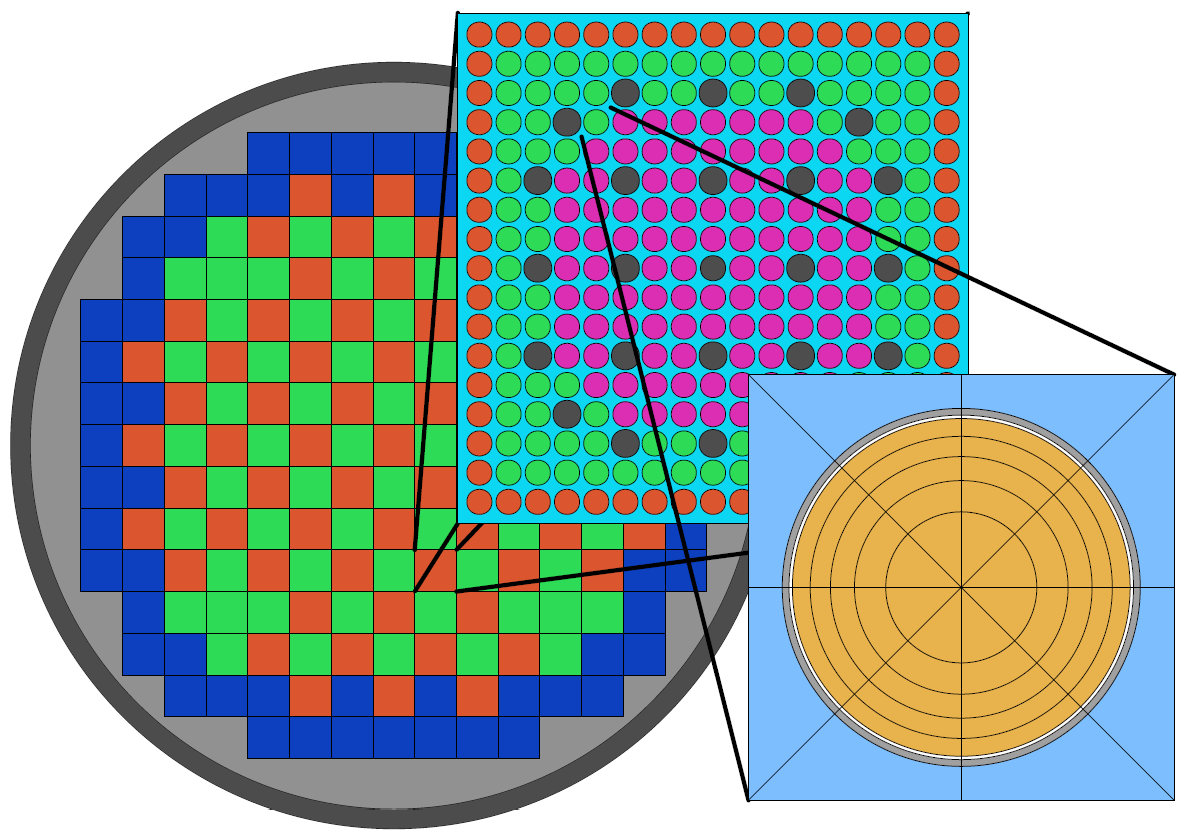
\includegraphics[width=0.7\textwidth]{reactor-geometry.png}
    \caption{Illustration of reactor geometry and mesh}\label{f:reactor-geometry}
\end{figure}

Most reactor analysis has historically used a two step approach.  The first step consists of lattice calculations.  These calculations are typically 2D transport calculations done on a single fuel assembly (center and right portions of Figure \ref{f:reactor-geometry}) to obtain a local shape for the flux distribution in that assembly.  This local distribution is used to homogenize cross sections for a global calculation, which would be done on a mesh similar to the leftmost part of Figure \ref{f:reactor-geometry}.  This second step generates the global neutron flux distribution for the entire reactor on a coarse mesh using diffusion calculations that are faster than transport calculations.  The global diffusion solution and the local transport solutions are then combined to reconstruct a global fine mesh solution that can be used for the necessary analysis.

While these methods have been sufficient for reactor design and operation to this point, the homogenization and reconstruction steps inherently introduce some uncertainty in the accuracy of the solution and are known to be inaccurate for some situations.  This uncertainty forces analysts to be conservative to account for the possibility that the code did not accurately predict the power distribution for a given fuel loading pattern or transient scenario.  This conservatism combined with a rapid increase in computing power in recent years has driven a push toward direct whole-core transport calculations.  These solutions require more computing resources to obtain, but are able to correctly model all the physics in the reactor in a single calculation and provide greater confidence in the solutions.

There are two categories of methods that can be used for transport calculations: Monte Carlo and deterministic.  Monte Carlo calculations use random sampling of (usually) continuous cross section data to determine the average behavior of neutrons throughout the reactor core.  Given enough time, a Monte Carlo calculation will give the exact solution.  However, the number of particles required to obtain a full core power distribution with acceptably low statistical uncertainty is prohibitive even with today's computing resources.  Deterministic calculations do not have to deal with statistical uncertainty and can provide solutions much more quickly than Monte Carlo calculations.  However, deterministic methods are limited by certain approximations and discretizations that adversely affect the accuracy of the solution.  Making improvements to these approximations is crucial to improving deterministic transport calculations and making them viable for practical reactor analysis.

\section{Motivation}

One category of whole-core deterministic transport methods that has gained popularity is planar synthesis methods.  Two types of planar synthesis methods under active research today are 2D/1D and 2D/3D.  In both of these methods, the reactor is modeled as a stack of 2D planes, which are then coupled through a second calculation.  Each 2D plane is solved using a high-fidelity transport method such as the method of characteristics (MOC).  In 2D/3D, these calculations are used to generate homogenized cross sections for a 3D discrete ordinates (S$_N$) calculation.  Because the MOC calculations are performed across the entire 2D plane, the homogenized cross sections are more accurate than any that can be produced by the traditional 2-step method.  If 2D/1D is used, the stack of 2D MOC solutions is coupled axially through a lower order diffusion or transport calculation in the axial direction.  This takes advantage of the fact that in many reactors, most heterogeneity is in the radial direction.  The solution changes shape much more slowly in the axial direction, so the same resolution is not needed as in the radial direction.

These planar synthesis methods are orders of magnitude faster than a full-core Monte Carlo calculation, but they are still much slower than traditional nodal methods used by industry.  To rectify this, it is important to improve the efficiency of these calculations to make them more useful for practical calculations.  Some of these efficiency gains can be realized by modifications to the methods and algorithms used in the codes.  However, a simpler way to reduce the runtime fo these calculations is to simply use a coarser mesh.  Because the most expensive part of the calculation is the 2D planar transport sweep, reducing the number of 2D planes can significantly reduce the computing resources required for the 2D/1D or 2D/3D calculations.

When reducing the number of 2D planes, care must be taken to ensure that no significant approximations are made.  These methods implicitly assume that there is not axial change in materials for a given 2D plane.  If this assumption is violated, these materials will be homogenized and introduce error in the solution.  For some models, explicitly meshing all axial components results in a relatively fine mesh, preventing any runtime reduction by coarsening the mesh.  To circumvent this issue, methods must be developed which are able to account for axial heterogeneity within a plane and preserve the accuracy of transport calculations without requiring a fine axial mesh.  The work presented here focuses on the development of such methods.

\section{Previous Work in 2D/1D}

Many different axial heterogeneities can be conjured up, but by far the most troublesome in most reactors is control rods.  Control rods move axially throughout reactor operation to control the power shape in the core, and they can move rapidly at times to maintain safe conditions during a transient scenario.  Furthermore, they tend to be strong neutron absorbers with relatively large cross sections.  Attempting to explicitly mesh every control rod position can result in an unusably fine axial mesh, but homogenizing the control rods axially within a plane results in unacceptably large errors in the flux distribution called rod cusping.  The application of subgrid methods developed in this work will be focused on the problem of rod cusping since it is the most severe axial heterogeneity for planar synthesis methods.

Rod cusping was first identified in \cite{finnemann1977RodCuspingOrigMention} in 1977 in the context of nodal methods.  In generating homogenized cross sections for the nodal calculation, it was discovered that simply having a rodded and unrodded version of the node cross section was insufficient and produced cusping errors.  Since then, a myriad of researchers have endeavored to resolve this issue \hl{citations galore}.  The rise of whole-core transport methods, including planar synthesis methods, addresses many shortcomings of the traditional reactor analysis codes, but not rod cusping \hl{citations}.

Methods to deal with control rod cusping up to this point have generally fallen into one of two categories: fast or accurate.  The fastest methods usually have pregenerated data from a separate set of calculations which can be used to quickly adjust cross sections for partially rodded nodes and improve the answers.  The most accurate methods reduce the rod cusping errors to levels that are usually acceptable, but enough additional calculation is required to achieve this accuracy that the methods are not much more beneficial than simply refining the axial mesh to eliminate the cusping altogether.  While some methods have bridged this gap between speed and accuracy better than others, none have succeeded at eliminating cusping altogether.  This work seeks to fundamentally resolve the control rods in the transport calculations in such a way that rod cusping errors are greatly reduced or eliminated without a significant increase in computational burden.

\section{Dissertation Overview}

This dissertation is organized into 5 main parts:

\begin{enumerate}
    \item Approximations and numerical methods used to solve the Boltzmann transport equation,
    \item An in-deptch description of the 2D/1D implementation used for this work,
    \item A detailed look at rod cusping and the history of decusping methods research,
    \item Descriptions of methods developed for this work, and
    \item Results and analysis of the newly developed methods.
\end{enumerate}

The first part will introduce the Boltzmann transport equation in its most general form.  The equation is continuous in space, energy, angle and time, so discretizations are required to solve the equation deterministically.  After discussing some of the common discretization schemes, some important numerical methods relevant to this work are discussed.  These include MOC, coarse mesh finite difference (CMFD), the spherical harmonics (P$_N$) approximation, and the collision probabilities (CP) method.  Detailed derivations are presented for those methods which will be modified as part of the new subgrid methods; other derivations are deferred to the appendices or external references.

After presenting the basic numerical methods, the following chapter will provide an in-depth look at the 2D/1D implementation in the MPACT code used for this research.  Some history of the method will be described first, followed by a derivation of the radial and axial equations used as a basis for the 2D/1D method.  The numerical methods and iteration scheme used by MPACT to solve these equations will then be described in detail.

With the foundation of 2D/1D laid, the third part will provide a more thorough discussion of rod cusping.  First, the cause and effects of the method will be described for both nodal and 2D/1D codes.  Second, a history of methods to resolve rod cusping will be discussed.  These methods will be grouped based on whether they were developed for nodal codes or 2D/1D codes.  This discussion will be used to more thoroughly motivate the need for advanced multigrid methods to address this problem.

Chapter \ref{chap:results} will describe the three new methods that have come out of this work.  These methods are described in increasing accuracy, complexity, and generality.  The first is polynomial decusping.  This method relies on pregenerated data to correct the cross sections in a partially rodded node prior to the beginning of the 2D/1D calculations.  This was developed primarily out of immediate need to address the rod cusping issue in MPACT.  The second method is called subplane collision probabilities.  This method modifies the axial part of the 2D/1D calculation to use a refined grid, then uses the CP method for the rodded and unrodded regions to generate improved flux shapes and cross sections.  This method is more general in its ability to handle multiple control rod types and other simple heterogeneities.  The final method is presented is a new version of MOC called subray MOC.  This method seeks to address axial heterogeneity during the 2D MOC sweeps, which should improve the solution at the most fundamental level instead of attempting to improve homogenized cross sections.

The final section will present results and analysis of the methods.  First, two problems will be presented to test the polynomial and subplane collision probabilities.  Both accuracy and runtime will be compared to reference cases with no rod cusping errors.  Second, results and analysis of subray MOC will be presented using another set of problems.  Accuracy, convergence, and runtime will be analyzed compared to reference cases.  Comparisons of subray MOC with the polynomial and subplane collision probabilities methods will also be made to show improvements in accuracy achieved by subray MOC.

The dissertation will close with a summary and brief discussion of future research topics related to the methods presented here.